

\section{Introduction}

%The memory management has a significant performance impact on the performance of applications, which could lead to as large as $9.7\times$ performance difference with different allocators. Figure~\ref{fig:motivation} evaluates the performance of five applications from two popular benchmark suite, PARSEC-2.0~\cite{parsec} and Phoenix~\cite{phoenix}, with the default Linux allocator (Glibc-XXX), TCMalloc-2.2, jemalloc-4.2.0, and Hoard-3.11. The figure shows that choosing a different allocator may cause the performance difference between 32\% faster to 9.7$\times$ slower.  

The performance of modern applications is often greatly impacted by memory accesses. when obtaining undesired performance, programmers mainly focus on optimizing the program code. Although memory allocators serve as the sole proxy for programs to request and return memory from the operating system, programmers lack even basic understandings of their behaviors, such as how well they perform themselves, how they interact with the OS, and whether their memory management policy fits the target program. 

Popular memory allocators indeed have dramatically different performance impacts on programs. Figure~\ref{fig:motivation} shows the normalized performance of ?? allocators on ?? benchmarks (details of the experimental setting in Section~\ref{sec:eval}) from two popular suites with ?? as the baseline. No allocators perform consistently the best across the benchmarks, and the largest performance gap of them on the same program is as large as ??X. For such cases, spending any additional effort of optimizing the user code will have the less impact than that of simply switching to a performant allocator.

\begin{figure}[!ht]
\centering
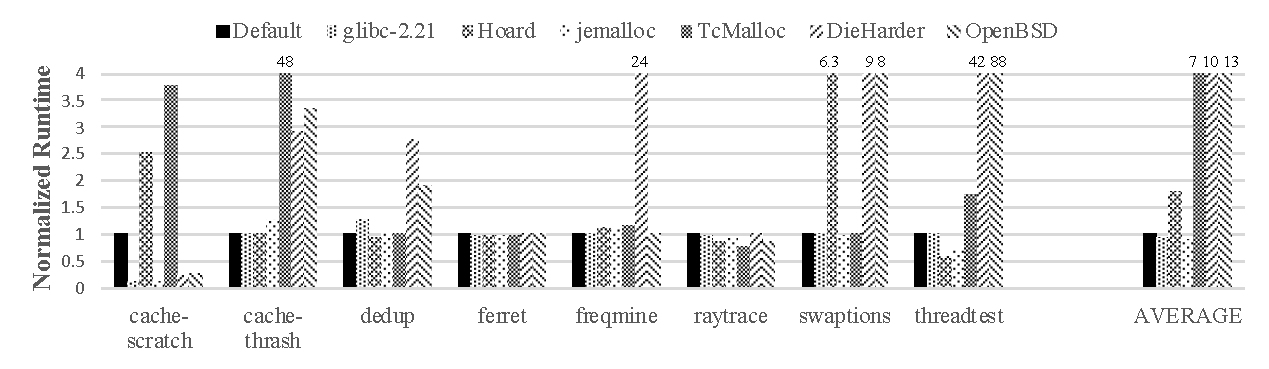
\includegraphics[width=3.3in]{figures/motivation}
\caption{Performance with Different Allocators\label{fig:motivation}}
\end{figure}

Unfortunately, there exist no profilers for programmers to understand the behavior of memory allocators in terms of their performance and memory impacts. Existing allocation profilers, such as \MP{}~\cite{Zorn:1988:MAP:894814}, \texttt{TCMalloc} Profiler~\cite{tcmalloc-profiler}, CLR profiler~\cite{lupasc2014dynamic}, or others~\cite{hirotaka2003developing}, mainly focus on how an application uses the memory,  instead of identifying the design problems of the allocators themselves. For instance, \texttt{mprof} may attribute memory allocations based to different allocation sites~\cite{Zorn:1988:MAP:894814}. The \texttt{TCMalloc} profiler reports program sites with a large number of allocations, locates memory leaks, and reports heap usage of any time~\cite{tcmalloc-profiler}. General profilers, such as gprof~\cite{DBLP:conf/sigplan/GrahamKM82}, Coz~\cite{Coz}, and perf~\cite{perf}, can not differentiate the performance issues caused by allocators and application code. Existing studies~\cite{Barroso:1998:MSC:279358.279363, Masmano:2006:CMA:1167999.1168012, ferreira2011experimental} simply compares the performance of different allocators, without revealing the underlying reasons. 

%Facing with this vast performance difference of different allocators, programmers may want to choose an appropriate allocator for their applications, in order to maximize the performance potential. Also, when facing performance degradation, they may also want to identify whether the degradation is caused by the allocator or not. For allocators designers, it is also extremely helpful to know the underlying reason of the performance slowdown (or speedup) of a specific allocator, so that they could further augment their design. All of these targets could be satisfied with an allocator profiler.  

In this paper, we propose \MP{}, the \textbf{first} general profiler to profile different memory allocators. \MP{} uses the hardware Performance Monitor Units (PMU) and RDTSC timestamps widely available in modern CPUs to perform the profiling. \MP{} achieves three goals to act as a practical memory allocator profiler for real-world programs. First, it should directly work on the executables. Second, it should reveal the overhead and scalability of the allocators themselves. Since the invocations to the memory management functions are synchronous, the efficiency of the allocator has a direct impact on performance. Third, it should quantify the ``application friendliness'' of the memory allocator, a metric to show how well the allocator manages memory for the application, which is drawn from statistics of accesses to different levels of the memory hierarchy.

%(1) When the profiler works directly on the executable, it is difficult to distinguish the behaviors caused by the allocators and those caused by the program code. 
% TP: I removed this, since it is too trivial, but they just didn't think about it. 
We face multiple challenges to achieve the goals. (1) The profiler, despite sampling a large number of events and obtaining extensive information, should maintain a low runtime overhead, and should not seriously distort the execution of the profiled targets (e.g. allocator).  (2) The profiler should not only identify the regular design issues (e.g., poor cache locality or poor object reuses) of the allocator, but also reveal the serious issue of interacting with the OS since a poor design may invoke excessive OS system calls and introduce unnecessary kernel contention. (3) A memory allocator may significantly affect the performance of applications, not just limiting to itself, which has never been evaluated quantitively before. (4) The profiler should be able to adapt to different allocators, which is the major target of designing a general profiler.   
%  to be quantified. 
% manage memory outside of its library calls, which is hard to capture and quantify. 
%carefully manage its internal memory allocations to

To address these challenges, we design \MP{} in a principled way to determine what events to sample and what profile knowledge the sampled events contribute to. Briefly speaking, \MP{} always intercepts the allocator library calls to figure out when the program execution is inside the allocator, during which it samples both performance related PMU events (e.g., cache misses) to determine the implementation issues and intercepts OS kernel calls to understand OS-level contention. When the program execution is outside of the allocator, \MP{} samples specific PMU events to determine cache line- and page-level utilization ratio, and cache contention rate, which could directly and significantly impact the performance of the corresponding applications. To maintain low overhead, \MP{} employs a fast lookup mechanism that enables fast checking on the size information of each object, and on the cache line usage and page usage upon each sampled access. ??(WB) one more sentence about the low overhead?? ??(WB) It allocates its internal memory on ...??

\MP{} successfully identifies several implementation issues located in popular allocators. For instance, \MP{} finds out that the DieHarder allocator causes excessive number of cache and TLB misses upon each deallocation, e.g. \todo{5 times} on average compared an optimized design. \MP{} reveals that multithreaded allocators, such as ??, reclaims memory but fails to reuse these freed memory for future requests, typically from another thread, which causes the blowup problem~\cite{Hoard}. \MP further shows that the ??allocator invokes different system calls, such as \texttt{mmap}, \texttt{brk}, \texttt{madvise}, and \textbf{munmap}, which cause unnecessary kernel contention inside the OS (and limit its scalability). Lastly, \MP{} evaluates the application friendliness of the allocators and show that the program's poor performance when using ?? is strongly correlated with its low friendliness. In all the profiling runs of real-world programs using popular allocators, \MP{} incurs at most ??X runtime overhead ??X memory overhead, while sampling and processing a large amount of events, and for the first time revealing various performance issues latent in the allocators.

%Basically, \MP{} utilizes the hardware Performance Monitor Units (PMU), RDTSC timestamp, and simple counters together to perform the profiling. For instance, it utilizes the RDTSC timestamps to collect the execution time of each allocation/deallocation, and utilize simple counters to obtain some statistics information, e.g. the number of allocations and deallocations, and so on. It also employs PMUs to collect  hardware events of each allocation and deallocation, such as TLB read/write misses, retired instructions, and page faults. Different from existing work, \MP{} proposes \textbf{the novel usage of PMUs to evaluate application friendliness}, such as cache utilization (and contention) ratio and page utilization ratio, which may indirectly affect cache misses and TLB misses. \MP{} samples memory accesses, and then obtains the cache utilization ratio and page utilization ratio in which each sampled access is located, and utilizes the sampled ratio to represent the overall ratio. Therefore, \MP{} could quantify the potential performance impact of a specific allocator on applications.    

However, there exists multiple implementation challenges. The most important challenge is the \textbf{overhead challenge}, where one careless design may impose up to 100 $\times$ overhead, based on our experience of the development. The huge overhead could be unaffordable even for development phases. More importantly, the significant overhead may skew the evaluation results unnecessarily. \MP{} takes multiple approaches to reduce the performance overhead. First, \MP{} designs a fast lookup mechanism that enables the fast checking on the size information of each object, and on the cache line usage and page usage upon each sampled access quickly, as further discussed in Section~\ref{sec:fastlookup}. This lookup mechanism is very difficult to design, since different allocators may have different behaviors, and their memory mappings are out of the control of \MP{} (without some obvious rules). Second, \MP{} minimizes the cache contention by utilizing thread-local recording, and only summarizing the data together in the end of execution. Third, \MP{} also reduces the allocation overhead of its recording data structures, by preallocating the space for internal memory usage. For instance, it employs the vast address space of 64-bits machines to design its lookup mechanism, and pre-allocates a huge space for saving the mapping. 

Another significant challenge comes from the adaption to different allocators. Specific issues include the following ones: (1) How to obtain the specific details of different allocators, such as size class information, type of allocator, metadata size information? (Section~\ref{}) (2) How to design the fast but general lookup mechanism for different allocators (Section~\ref{})? There are multiple factors may affect the design: the default Linux allocator extends its heap differently with the \texttt{sbrk} system call, making one of its heap arena far from other arenas (making it difficult to design the virtual memory)? Secure allocators, such as OpenBSD and DieHarder, may invoke one \texttt{mmap} to obtain one page from the OS. That is, there are a large number of mappings inside the OS. This fact makes some general data structures not suitable to support the fast lookup, such as a hash map or the range tree. (3) How to measure the kernel contention inside the OS (Section~\ref{})? The Linux's glibc-2.21 has a very serious performance problem that is caused by the kernel contention, due to its careless invoking of system calls (\texttt{madvise}). (4) How to measure the user-space contention for the Glibc's allocator (Section~\ref{})? 

\begin{comment}
Challenge 2: how to perform the profiling? Similar to existing work, we majorly use the time (supported by RTDSC), the number (instrumentation-based counting), and some hardware events (PMU events) to perform the sampling. The sampling approach will be similar to existing work, but we attribute those events to the memory management events, such as allocations and deallocations. 

Challenge 3: how to reduce the performance overhead? In order to reduce the number of cache contention, we re-design our data structure to avoid false sharing and true sharing as much as possible. Also, we 

Challenge 4: we propose a novel method to evaluate the application friendliness. We evaluate the cache friendliness, or TLB friendliness. 

Challenge 5: we employs an internal allocator to avoid the interfering with allocations and deallocations of applications.  

 
\MP{} utilizes multiple methods to minimize the performance overhead of the profiling.  

\end{comment}

\MP{} also avoids the pollution on the profiling data. For instance, since \MP{} is designed to profile the allocators on specific applications, its internal memory allocations should be separated from those  of applications. \MP{} avoids the change of different allocators by intercepting allocations/deallocations and system calls through the preloading mechanism, which makes it a drop-in library. Overall, \MP{} only introduces around $2\times$ performance overhead and around $3\times$ memory overhead, while providing abundant information about allocators itself. During its experimentation, \MP{} is employed to discover various issues of existing popular allocators. It further presents the first quantitative comparisons on different allocators, not limiting to the external performance comparison on different applications.  

%\MP{} is also adapted to different allocators, which employs a  test program to obtain the details of different allocators, such as the type of the allocator, size class information, and the metadata overhead of each object. 


\begin{comment}

1. Maybe we should detect the contention rate. If the last write is from a different thread, we will detect one contention. 
 
allocator: can we use some different configurations of the same allocator?
Can we use the same allocator on different applications, achieving different allocators?  
}





performance overhead: 
1. Using the hash maps to identify the size of each object is very slow. 
2. Turning multiple reads into one read around 2 or three times. 
3. Using the new mapping mechanism. 

How we can do that for glibc. We migrate the glibc as separate library, allowing us to intercept system or libraries. 

How to figure out the metadata information?
	
\end{comment}

 



\begin{comment}

Challenge 1: How to know the specific details of different allocators? We utilized a small program to get the allocator's specific feature. For instance, whether they are BIBOP style or Bump-pointer based, the size class information and the metadata information. 

Challenge 2: how to perform the profiling? Similar to existing work, we majorly use the time (supported by RTDSC), the number (instrumentation-based counting), and some hardware events (PMU events) to perform the sampling. The sampling approach will be similar to existing work, but we attribute those events to the memory management events, such as allocations and deallocations. 

Challenge 3: how to reduce the performance overhead? In order to reduce the number of cache contention, we re-design our data structure to avoid false sharing and true sharing as much as possible. Also, we 

Challenge 4: we propose a novel method to evaluate the application friendliness. We evaluate the cache friendliness, or TLB friendliness. 

Challenge 5: we employs an internal allocator to avoid the interfering with allocations and deallocations of applications.  


Overview:
\MP{} is an drop-in library that should be linked before any runtime library. Similar to existing profilers, \MP{} also collects  hardware events, time information and the number of invocations. However, \MP{} attribute these events or data to each invocation of memory allocation and deallocation, which can present users  intuitive information about the possible issue of each allocator. As a profiler, \MP{} further summarizes the performance overhead, memory overhead, scalability, and application friendliness of each allocator. 


For performance overhead, \MP{} focuses on the following items: 


Since memory overhead can be caused by multiple factors, such as metadata overhead, alignment overhead (internal fragmentation), and memory blowup. Memory blowup is defined as ,. 

For scalability, \MP{} not only focuses on the potential bottleneck within the user space, but also includes the potential bottleneck caused by the allocator. Programmers have identified one particular performance bottleneck of applications, such as dedup issue. 
It won't cause the . 

\MP{} also aims to answer whether an allocator is friendly to the applications or not, such as . . 


   


MallocProfiler will serve two purposes. 
(1) This will be utilized to get the allocator related parameters. 

(2) We will be able to identify whether the performance problem is caused by the memory allocator. We could actually divide the overhead to the overhead of allocator or the overhead of applications. 
Therefore, we could identify the root causes and not always blame for the application writer. 



 

However, the memory allocator itself has not got sufficient attention that it should reserve to. 
For instance, there is no an dedicate the allocator profiler that can be utilized for identify the allocator's behavior.

Having this profiler will serve three purposes. First, it will help the designers and developers that could discover the issues of memory allocators, without the need of porting or developing the profiler for a specific allocator. Second, it helps programmers to determine whether the performance issue is coming from the memory allocator. Third, it will help users to choose the best memory allocators that is suitable for a specific applications, if there are multiple choices available. 

 Linux, TCMalloc, Jemalloc, Hoard, OpenBSD, DieHarder. Then shows the internal reason of why some are slower than others. 

We may choose two general-purpose allocators and two secure allocators. Then we know why secure allocators are slower, currently. 

The general idea is to understand performance, memory, and scalability of different allocators, while providing some evidence of allocator. During the design of allocator, we usually need to understand the inherent reason. The difficulty is how to collect the information without changing the specific allocator. That is, how to design a general allocator profiler, which can help assist the analysis of different allocators. 

We will work on the allocator profiling to understanding the performance, memory and scalability of memory allocator. We may  memory related those system calls. How long it spent on the memory allocation and deallocation, using RDTSC, which can be caused by long memory allocation time? How much of objects has been re-utilized? How is the memory blowup, what is the memory consumption and how much has been allocated? Can we know lock contention of memory allocation, maybe we could monitor the lock usage, just as SyncPerf, and identify that lock acquisitions are  waiting during allocation? Can we identify is there inter-objects cache contention on these objects? If yes, that is the possible example of these allocators.  

What are the design goals of \MP{}? 

\MP{} needs to be general to different memory allocators, which requires no change of the code at all even when connecting with different allocators. The first target is transparency, which should not require the changes of allocators, if the allocator is working as a dynamic library. 

Second, \MP{} should be able to identify the issues of different allocators. 


	
\end{comment}


\begin{comment}

Dynamic memory management plays an important role in the performance of applications, especially on multithreaded programs. 
For performance related to memory uses, some work focuses on improving existing memory allocators. Some focuses on a better memory layout among different elements of the same data structure. 
But there is little work that focuses on the improving the performance by changing the behavior of memory allocations and deallocations. 

\HeapPerf{} tries to identify some places inside applications that can introduce the performance problems. These problems can be solved by changing the behavior of memory allocations, without using the new memory allocator. 
These problems are rarely investigated in the past. The most closest work related to this is to simply record the placement with excessive allocations. However, excessive allocations is a total class of the problems that are investigated in this paper, but the existing work fails to present any detailed idea on the following problems: whether all these excessive memory allocations can be reduced? whether they can improve the performance? how to reduce that? These questions requires highly expertise and large amount of manual effort. Instead, \HeapPerf{} presents more useful idea on these questions, and hope to guide programmers, even non-experts, to solve these problems easily. 

We observe three different patterns that can cause performance problems, or called as anti-patterns~\cite{}. 

The second type is shown as Figure~\ref{}. In this example, there are a number of memory allocations that will allocate small amount of bytes for each one. More particularly, these allocations are inside the same loop, and have the same size. Unfortunately, memory allocators will not precisely allocate the specified size of objects. For example, the \texttt{glibc} allocator will allocate 32 bytes as long as the required size is between 4 bytes and 24 bytes. Based on the explanation of Hoard~\cite{Hoard}, this method helps to manage small sizes of different objects, without introducing too many external fragmentation. However, this also introduces a significant problem on cache inefficiency, since only less than 13\% cache is actually utilized, which can introduce around $8\times$ performance slowdown comparing to the code listed in Figure~\ref{}. 


The second type is shown as Figure~\ref{}, there are a number of unnecessary memory allocations and deallocations. By moving the placement of allocations to outside the loop, we can significantly improve the performance by reducing the overhead related to memory allocations and deallocations. 

The third type is related to the uses of heap variables or stack variables. Some excessive heap objects, if they are turned into stack variables, will have large performance benefit. Comparing to heap objects, the overhead of memory allocations and deallocations can be largely reduced if using stack variables. Also, the stack is typically locate inside the cache, which will have lower access latency. Also, stack variables will have exact size, without the addition of metadata and huge alignment. 
\todo{Whether those variables have been touched only very few times, typically should be putted into the heap objects since they may cause the in-efficient cache utilization as well}.  
 


Heap memory related performance bugs can be from the following categories, if only think about applications. 

\begin{itemize}
\item: Too many allocations and deallocations. The total run time spending in memory allocation and liberation may take up to 30\% execution time\cite{1190248}. 

\item: Too many memory uses: this can actually affect the performance when there are too much memory that has been allocated but not used. This can be caused by memory leaks or too late de-allocation. \todo{Most existing tools focus on the memory leak, but whether there are some tools that can uncover delayed-deallocation?}  

\item: 
\end{itemize}


What we can do for heap memory management?

First, we can point out the unnecessary memory allocations and deallocations. For example, we can malloc a large object, and then assign to different small projects. Some of them may be called inside the internal level of loop functions, we can move up to external loop level. 
By reducing unnecessary memory allocations, we expect to improve the performance. 

Second, we can give a statistics on the life-span of objects. Whether we can find out some problems inside? For example, we can use stack variables instead of heap if some objects are too short-lived, or mostly inside a function call. 

Third, we can actually give the statistics on each callsite. Some callsites may have larger number of allocations. 

Can we evaluate the performance related to heap allocations? For example, how much time is spending on memory allocation. 
We can approximate the time of spending on each allocation. Then we can attribute the time to different statements, just similar to gprof. Then maybe it is obvious that we can reduce the overhead by reducing the memory allocations. Then it is possible that a separate paper by using the 


In the end, although not every interested, it is to check the overhead of every memory allocation on each popular memory allocation. Thus, pointing out that the memory allocation actually should pay attention to the level of stacks. Thus, it is possible that we can design a new memory allocator by reducing the level of memory allocation. This is a reverse to HeapLayer. It is great to have an survey paper on this:

A. How is the overhead of memory allocation in large applications? How we can evaluate it? 
B. How is the overhead that comes from memory management? We evaluate this on some popular benchmarks. 
C. Whether the overhead comes from different cache uses? or other things. 
D. It will shed a light whether we need to re-design the memory allocator. 
It will be a perfect paper for ICSE or SC.

How we can evaluate the cache friendliness of memory allocators? 
For instance, how much memory will be reutilized immediately? If one direct use will be one point, then how many score of different allocators. 

Also, how much of memory blowup? 

%%%%%%%%%%%%%%%%%%%%%%%
% Possible solutions:
% (1) We will check the malloc and free are allocated in sequence. For example, we are always doing the malloc(8) and free(8) in sequence. Given the number of these allocations is large. Then it is much possible that it is a problem. However, it can be a problem for the performance reason. But we can basically maintain a stack that maintains five possible allocations. 
%% Should we just use a two-phase solution? That is, we can use a hash-table to identify different allocation site with their memory uses: how many times for memory allocations? How many times for related free operations? If there are a lot of memory allocations that are not freed, then it is possible a memory leak. We could also identify whether those memory are actually touched or not by using the watchpoint mechanisms? Also, we may try to check whether memory allocation are in the same sequence, for example, alloc-free-alloc-free, and with the same size. If yes, then it is possible that is unnecessary memory operations. 

%%%%%%%%%%%%%%%%%%%%%%%%%
Typically, I think that mtrace utilizes 

Can we check the example of malloc-free situations?
Can we base on a ``anomaly detection'' but.  
I guess that the memory will be freed before the next allocation. If not, then there is high probability of leaking. If memory allocated is on the same site, 
	
\end{comment}
 
\MP{} will help programmers and users in the following aspects. First, it helps designers and developers of memory allocators to  discover potential issues of a memory allocator, without the requirement of developing a custom profiler. By providing the detailed comparison between popular allocators, the paper also provides some insights and guidelines about the allocator design. 
  Second, it helps programmers to determine whether the performance/scalability issue is coming from the memory allocator. Third, it helps users to choose the best memory allocators for a specific applications, if there are multiple choices available. Fourth, it also helps users discover some potential issues related to  memory allocations, such as excessive memory consumptions.  



\subsection*{Contribution}

Overall, this paper makes the following contributions. 

\begin{itemize}
\item It designs and implements \textbf{the first general profiler}--\MP{}--to profile different aspects of different memory allocators, without changing allocators themselves.  

\item \MP{} employs advanced hardware, such as Performance Monitoring Units (PMU) or Read Time-Stamp Counter (RDTSC), and simple counters together to profile allocators quantitatively. \MP{} attributes the data to each allocation and deallocation, helps discover some issues that cannot be discovered with general profilers.  
%Overall, it can not only pinpoint the major issues inside the implementation of memory allocators, such as performance, memory, and scalability issues, but also could quantitively pinpoint cache or page utilization issues of allocators.  

%\item \MP{} proposes the employment of hardware PMUs to evaluate performa metrics efficiently and effectively. 

\item This paper performs extensive experiments on multiple memory allocators. It pinpoints some performance or memory issues latent in existing allocators. It also provides the first quantitative comparison of different factors of multiple widely-used allocators.  

\end{itemize} 


\todo{What is new in this tool? Whether it could provide some information that is not available in an existing allocator.}

\begin{itemize}
\item It will provide the application friendliness that is not available in existing work, which helps users to decide which allocator should be used for the specific allocator. 
\item It will provide the memory usage (overhead) information, such as internal fragmentation, and objects that are not freed but not used at all. 
\item It will provide some information that only exists in multiple profilers, for instance, the average number of instructions of each allocation and deallocation, the average time spending in each allocation and deallocation (PMU sampling will be placed outside the time spanning), (not how long this allocation and deallocation has been sampled), whether there are some contentions during allocation (user space and kernel space), how many lock acquisitions.  
\end{itemize}
 
\subsection*{Outline}

The remained of this paper is organized as follows. Section~\ref{} discusses the overall design purpose of \MP{}, and Section~\ref{} presents the detailed implementation. Section~\ref{} shows the results of experiments on different allocators using \MP{}. Then Section~\ref{} discusses related work in this field, and Section~\ref{} concludes this paper. 